\documentclass[tikz]{standalone}
\usepackage{xcolor}
\definecolor{coilcolor}{rgb}{0.8,0.5,0.5}
\definecolor{photoncolor}{rgb}{0.65, 0.16, 0.16}
\usetikzlibrary{decorations.pathmorphing,calc}


\newcommand{\AxisRotator}[1][rotate=0]{%
    \tikz [x=0.25cm,y=0.60cm,line width=.1ex,-stealth,#1] \draw (0,0) arc (-150:150:1 and 1);%
}
\begin{document}
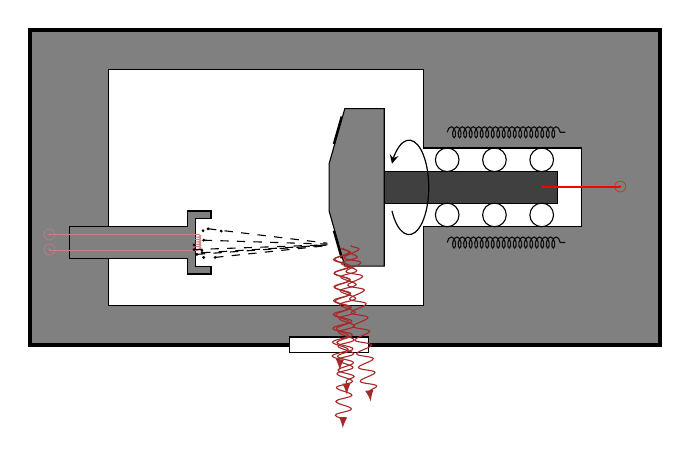
\begin{tikzpicture}
	\draw [ultra thick, fill=white!50!black] (-4, -2) rectangle (4, 2);
	\draw [fill=white] (-3, 1.5) -| ++(4, -1) -| ++(2, -1) -| ++(-2, -1) -| cycle;
	\draw [fill=gray] (0, 1)  -| ++(0.5, -2) -- ++(-0.5, 0) -- ++(-0.2, 0.7) -- ++(0, 0.6) -- cycle;
	\draw [thick] (-0.04, 0.9) -- ++(-0.1, -0.35);
	\draw [thick] (-0.04, -0.9) -- ++(-0.1, 0.35) node [midway] (a) {};
	\draw [fill=gray!50!black] (0.5, 0.2) -| ++(2.2, -0.4) -| cycle;
	\draw [fill=gray] (-3.5, -0.5) -- ++(1.5, 0) -- ++(0, 0.2) -- ++(0.3, 0) -- ++(0, -0.1) -- ++(-0.2, 0) -- ++(0, -0.6) -| ++(0.2, -0.1) -| ++(-0.3, 0.2) -| cycle;
	\draw [coilcolor, local bounding box=coil, decoration={segment length=0.3mm, amplitude=0.2mm,coil},decorate] (-1.85,-0.6) -- ++(0, -0.20);
	\draw [coilcolor] (coil.north) -- (coil.north -| -3.75, 0) node {\tiny \(\odot\)};
	\draw [coilcolor] (coil.south) -- (coil.south -| -3.75, 0) node {\tiny \(\odot\)}; % node [black, scale=0.5, text width=2cm, left=-0.5cm] {Cathode Voltage};
	\draw [decoration={segment length=0.7mm, amplitude=0.7mm,coil},decorate,opacity=0.9] (1.3,-0.7) -- ++(1.5, 0);
	\draw [decoration={segment length=0.7mm, amplitude=0.7mm,coil},decorate,opacity=0.9] (1.3,0.7) -- ++(1.5, 0);
	\node at (0.85,0) {\AxisRotator};
	\draw (1.3, 0.35) circle (0.15);
	\draw (1.9, 0.35) circle (0.15);
	\draw (2.5, 0.35) circle (0.15);
	\draw (1.3, -0.35) circle (0.15);
	\draw (1.9, -0.35) circle (0.15);
	\draw (2.5, -0.35) circle (0.15);
	\draw [fill=white] (-0.7, -1.9) rectangle ++(1, -0.2);
	\draw [thick, red] (2.5, 0) -- ++(1, 0);
	\node [red] at (3.5, 0) {\tiny \( \odot \)};
	\def\coordrand{0.1}
	\def\rayrand{0.5}
	\foreach \raand in {1,...,4}
	{
		\draw [
			-latex, decorate, decoration={snake, amplitude=0.1cm, segment length=5pt, post length=1mm},%
			color=photoncolor
		] ($(a) + (\coordrand * rand + 0.07, \coordrand * rand)$) -- ++($(-0.2, -2) + (\rayrand * rand, \rayrand * rand)$);%
	}
	\def\erand{0.2}
	\foreach \raand in {1,...,11}
	{
		\coordinate (e\raand) at ($(coil.east) + (\erand * rand + 0.08, \erand * rand)$);
		\fill (e\raand) circle (0.02);
		\ifodd\raand
		\draw [dashed] (e\raand) -- (a);
		\fi
	}
\end{tikzpicture}
\end{document}
